\section{Data, availability and evidence accounting}\label{sec:section-03}

\subsection{Universe and provider snapshots}

The verified market panel contains 55,242 instrument-session observations on 2,511 common market dates. There are 686 recorded decision dates, 680 with mature outcomes, and 132 instrument-date predictions whose outcomes are unavailable at the historical cutoff. The inherited release reports 726 refits. The inventory rechecked 722 preserved files and directly compared 66 saved reproduction outputs. These are new integrity checks of saved records, not a claim that all old models were trained again.

The universe was inherited from the project rather than sampled from historical index constituents. It mixes individual surviving companies, broad-market funds, sector funds and alternative-asset funds. Economic exposures overlap: holding a growth stock and a fund that contains it does not create two independent bets. The declared growth-group limit captures only one part of that overlap. We cannot estimate delisting bias from this universe, and we do not interpret the results as a market-wide stock-selection claim.

Raw provider OHLCV and adjusted series are separate artifacts. The term raw refers to the provider's returned fields before this pipeline's adjustment transformation; it does not certify an archival, unadjusted exchange tape. Adjusted prices incorporate the vendor's present interpretation of splits and distributions. Each snapshot records retrieval time and hashes. Historical availability uses an explicit completed-session convention because the provider does not supply an immutable historical arrival timestamp for every bar. A current-vintage reconstruction is not equivalent to a point-in-time archive.

For the local simulation, quantities are total-return proxy units. Future provider revisions can rescale historical adjusted prices, so daily marks chain the newly observed adjusted return onto stored marks. That convention avoids treating a uniform rescaling as a windfall or loss in existing holdings. It does not implement broker shares, dividend cash payments, fractional-share restrictions or corporate-action entitlements. Raw responses and available action events are retained for provenance, while broker accounting remains a separate unimplemented contract.

\noindent Table~\ref{tab:1} reports dataset flow; counts are instrument-dates unless the stage explicitly says dates.

\begin{table}[!htbp]\centering\footnotesize\setlength{\tabcolsep}{3pt}\renewcommand{\arraystretch}{1.14}
\caption{Dataset flow; counts are instrument-dates unless the stage explicitly says dates}\label{tab:1}
\begin{tabular}{@{}>{\raggedright\arraybackslash}p{\dimexpr 0.82819\textwidth-3.000pt\relax}>{\raggedleft\arraybackslash}p{\dimexpr 0.17181\textwidth-3.000pt\relax}@{}}
\toprule
\textbf{Stage} & \textbf{Count} \\
\midrule
raw\_\allowbreak{}symbol\_\allowbreak{}sessions & 55,242 \\
common\_\allowbreak{}market\_\allowbreak{}dates & 2,511 \\
feature\_\allowbreak{}complete\_\allowbreak{}symbol\_\allowbreak{}sessions & 49,698 \\
warmup\_\allowbreak{}symbol\_\allowbreak{}sessions & 5,544 \\
pre\_\allowbreak{}evaluation\_\allowbreak{}feature\_\allowbreak{}complete\_\allowbreak{}symbol\_\allowbreak{}sessions & 34,606 \\
decision\_\allowbreak{}symbol\_\allowbreak{}sessions & 15,092 \\
mature\_\allowbreak{}labeled\_\allowbreak{}symbol\_\allowbreak{}sessions & 14,960 \\
unmatured\_\allowbreak{}symbol\_\allowbreak{}sessions & 132 \\
\bottomrule\end{tabular}\par\smallskip
\raggedright\textit{Source:} \path{data/research-v2/tables/diag_dataset_flow.csv}.
\end{table}


\noindent Figure~\ref{fig:1} shows coverage, retained observations and class support from the saved panel.

\begin{figure}[htbp]\centering
% Native editable figure; frozen statistics 0d291b4aebf8c524dc6705d872c070feb990e86a1cebbd59a758f400b240c952
\begin{minipage}[t]{.48\linewidth}\centering
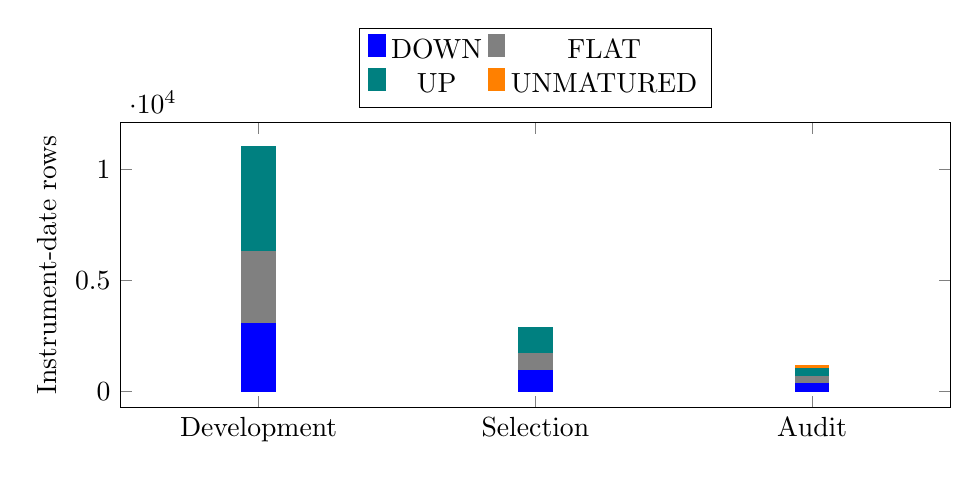
\begin{tikzpicture}
\begin{axis}[width=\linewidth,height=5.2cm,ybar stacked,bar width=12pt,xtick={0,1,2},xticklabels={Development,Selection,Audit},ylabel={Instrument-date rows},legend columns=2,legend style={at={(0.5,1.05)},anchor=south},enlarge x limits=.25]
\addplot+[blue,fill=blue,draw=blue] coordinates {(0,3081) (1,952) (2,351)};
\addlegendentry{DOWN}
\addplot+[gray,fill=gray,draw=gray] coordinates {(0,3230) (1,768) (2,326)};
\addlegendentry{FLAT}
\addplot+[teal,fill=teal,draw=teal] coordinates {(0,4733) (1,1140) (2,379)};
\addlegendentry{UP}
\addplot+[orange,fill=orange,draw=orange] coordinates {(0,0) (1,0) (2,132)};
\addlegendentry{UNMATURED}

\end{axis}
\end{tikzpicture}
\end{minipage}
\hfill
\begin{minipage}[t]{.48\linewidth}\centering
\resizebox{\linewidth}{!}{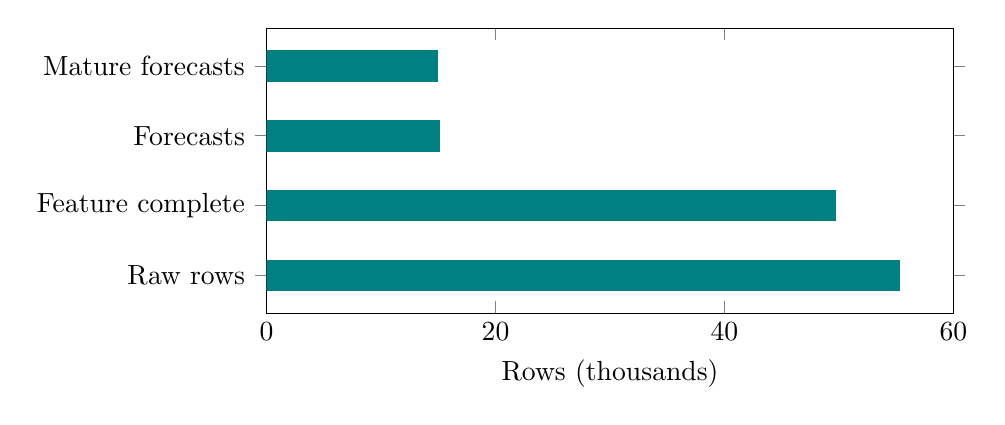
\begin{tikzpicture}
\begin{axis}[width=.85\linewidth,height=5.2cm,xbar,bar width=11pt,ytick={0,1,2,3},yticklabels={Raw rows,Feature complete,Forecasts,Mature forecasts},xlabel={Rows (thousands)},enlarge y limits=.18,xtick={0,20000,40000,60000},xticklabels={0,20,40,60},xmax=60000,scaled x ticks=false,x tick label style={/pgf/number format/fixed},xmin=0]
\addplot+[teal] coordinates {(55242,0) (49698,1) (15092,2) (14960,3)};
\end{axis}
\end{tikzpicture}
}\end{minipage}
\caption{Coverage, retained observations and class support from the saved panel.}\label{fig:1}
\end{figure}

\subsection{Admission, missingness and labels}

Every admitted price panel must have unique, monotonically ordered session keys, finite positive OHLC values, valid high/low ranges and positive observed volume. The exchange calendar, rather than a generic weekday index, defines expected sessions. There is no holiday padding, synthetic zero-volume bar, stale-price forward fill or silent fallback to the last successful forecast. An unavailable bar stops the applicable batch before account decisions. Dropping a record, skipping an event and predicting FLAT are different states and remain distinguishable in the evidence.

For information observed at the end of session t, the first modeled fill is the next completed close. The target return is therefore:

\begin{equation}\label{eq:target}r^{\mathrm{target}}_t=\frac{C_{t+6}}{C_{t+1}}-1.\end{equation}

A return below -1\% is DOWN, above +1\% is UP, and an observed return between those thresholds is FLAT. A target whose ending close has not occurred is unobserved, not FLAT. Strict fitting eligibility requires its endpoint to precede the refit decision. The distinction matters twice: at the tail of the study, where decisions outnumber mature labels, and at partition boundaries, where adjacent labels can otherwise reveal later evaluation prices.

Dataset accounting is performed separately for price rows, usable feature rows, decision rows, label-complete instrument-dates and account sessions. A portfolio needs marks even when an outcome label is not yet mature. Thus the last account sessions legitimately contribute to equity measurement while being excluded from classification. The tables and claim map preserve those denominators instead of calling every row a sample with independent statistical information.

\subsection{Exposure log and optional information}

All historical dates inspected in the prior tasks or saved release are listed in the evaluation-exposure log. The old development, selection and audit labels are retained as names for reproducible date ranges, not as a claim that the current analyst is blind to them. The new controlled experiments use development-era chronological blocks and do not replace the previously selected prospective shadow. Historical results are useful for diagnosing a design and measuring its behavior; independent confirmation must come from later observations under a frozen rule.

Macro, news and crypto are excluded from the primary information set. A working public endpoint does not establish historical vintage eligibility. Revised macro observations need release/vintage timestamps; news requires retained content, version and availability times; a bounded recent crypto endpoint does not supply the requested long archive. Legacy XGB, LGBM, LSTM, MoE and zoo outputs remain preserved. Their different targets, information sets and splits prevent treating their old headline scores as controlled architectural comparisons. The registry records scope exclusions rather than silently dropping weak models.
